\documentclass[11pt, a4paper]{book}
\usepackage[french]{babel}
\usepackage[utf8]{inputenc}
\usepackage{answers}

\usepackage{hyperref}
\usepackage{multicol}

\usepackage[table,xcdraw]{xcolor}
\usepackage{listings}
\definecolor{ForestGreen}{RGB}{34,139,34}


\usepackage{enumitem}

\AtBeginDocument{\def\labelitemi{$\bullet$}}


\newcommand{\py}{\lstinline{Python} }


\definecolor{backcolour}{rgb}{0.95,0.95,0.92}

\lstset{%
	language         = Python,
	backgroundcolor  = \color{backcolour},
	basicstyle       = \ttfamily, % \upshape\ttfamily,
	keywordstyle     = \bfseries\color{blue}, %\bfseries,
	stringstyle      = \color{magenta},
	commentstyle     = \color{ForestGreen},
	alsoletter = > ,
	morekeywords = {>>>,as,assert,False,None, nonlocal,True, with,yield , <<, >>, :},
	showstringspaces = false,
	numbers=left,
	stepnumber=1,
	literate={à}{{\`{a}}}1 {é}{{\'e}}1 {è}{{\`{e}}}1 {ê}{{\^{e}}}1 {Ê}{{\^{E}}}1 {î}{{\^i}}1 {ô}{{\^{o}}}1 {ç}{{\c{c}}}1 {Ç}{{\c{C}}}1
}

\newcommand{\itemb}[1]{\item \textbf{#1}}

\usepackage{fancyhdr}  %package pour en-tetes et pied de pages
\usepackage{sectsty} % Permet de faire des modifications de police dans diverses sections des "headings" (cf. modif presentation de la page)
\pagestyle{fancy}       %Style pour en-tetes et pieds de pages
\fancyhead[CO,CE]{\sc Série 1\hspace{0.5mm}}
\fancyhead[RO,LE]{Collège Sismondi}  % LaTeX/TEX define \strut to be an invisible box of width zero that extends just enough above and below the baseline. Cela permet d'augementer légèrement la taille en bas de la box de manière à ce qu'elle soit collée à la ligne.
\fancyhead[LO,RE]{\small\ \textsl{1\textsuperscript{ère} année - DO Informatique}}
\fancyfoot[RO,LE]{2021 - 2022}
\fancyfoot[LO,RE]{\small }
\fancyfoot[CO,CE]{\thepage}

\fancyhfoffset[l]{1.2cm} % le "l" en paramètre permet d'indiquer qu'on ne veut modifier que la marge à gauche.
\renewcommand{\headrule}{{%
		\hrule \headwidth \headrulewidth \vskip-\headrulewidth}}
\renewcommand\footrulewidth{\headrulewidth}
\renewcommand{\footrule}{{%
		\vskip-\footruleskip\vskip-\footrulewidth
		\hrule \headwidth \footrulewidth\vskip\footruleskip}}

\usepackage{tikz}
%-------------------------------------------------------------------------------
%---- Eclairage : en encadré sur fond jaune avec symbôle "ampoule" à gauche ----
%-------------------------------------------------------------------------------
\definecolor{coleclairage}{RGB}{255 , 221 , 156}
\definecolor{contoureclairage}{RGB}{255 , 192 , 0}
\newenvironment{eclairage}
{
	\begin{center}%
		\begin{tikzpicture}%
			\node[rectangle, draw=contoureclairage, top color=coleclairage!50, bottom color=coleclairage!140, rounded corners=5pt, inner xsep=5pt, inner ysep=6pt, outer ysep=10pt]\bgroup                     
			\begin{minipage}{0.98\linewidth}
				\begin{minipage}{0.08\linewidth}\centerline{
\includegraphics[scale=1]{Symbole_eclairage.png}}\end{minipage}
				\begin{minipage}{0.89\linewidth}\itshape\footnotesize
				}
				{                		
				\end{minipage}
			\end{minipage}\egroup;%
		\end{tikzpicture}%
	\end{center}%
}

%-------------------------------------------------------------------------------
%---- apprendre : en encadré sur fond jaune avec symbôle "ampoule" à gauche ----
%-------------------------------------------------------------------------------
\definecolor{colapprendre}{RGB}{50,205,50}
\definecolor{contourapprendre}{RGB}{34,139,34}
\newenvironment{apprendre}
{
	\begin{center}%
		\begin{tikzpicture}%
			\node[rectangle, draw=contourapprendre, top color=colapprendre!10, bottom color=colapprendre!50, rounded corners=5pt, inner xsep=5pt, inner ysep=6pt, outer ysep=10pt]\bgroup                     
			\begin{minipage}{0.98\linewidth}
				\begin{minipage}{0.08\linewidth}\centerline{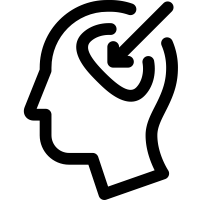
\includegraphics[width=30px]{Symbole_learn.png}}\end{minipage}
				\begin{minipage}{0.89\linewidth}\itshape\footnotesize
				}
				{                		
				\end{minipage}
			\end{minipage}\egroup;%
		\end{tikzpicture}%
	\end{center}%
}

\definecolor{colimportant}{RGB}{247 , 189 , 164}
\definecolor{contourimportant}{RGB}{237 , 125 , 49}
\newenvironment{important}
{
	\begin{center}%
		\begin{tikzpicture}%
			\node[rectangle, draw=contourimportant, top color=colimportant!50, bottom color=colimportant!140, rounded corners=5pt, inner xsep=5pt, inner ysep=6pt, outer ysep=10pt]\bgroup                     
			\begin{minipage}{0.08\linewidth}\centerline{
\includegraphics[scale=0.8]{Symbole_attention.png}}\end{minipage}
			\begin{minipage}{0.89\linewidth}
			}
			{                		
			\end{minipage}\egroup;
		\end{tikzpicture}%
	\end{center}%
}

%-----------------------------------------------------------------
%---- Modification présentation de la page: marges de la page ----
%-----------------------------------------------------------------
%\addtolength{\hoffset}{-1in}              % 1
%\addtolength{\voffset}{-1in}              % 2
\addtolength{\oddsidemargin}{-0.1 in} % 3
\addtolength{\evensidemargin}{-1in} % 3
\addtolength{\topmargin}{-1in}       % 4
\addtolength{\headheight}{6pt}       % 5
%\addtolength{\headsep}{-0.2cm}           % 6
\setlength{\textheight}{26cm}    % 7
\setlength{\textwidth}{16.5cm}      % 8
\addtolength{\marginparsep}{0pt}      % 9
\setlength{\marginparwidth}{0pt}   % 10
\addtolength{\footskip}{-1mm}           %11

\setlength{\parindent}{0em}% pas d'indentation


% Customiser le nom des sections
\usepackage{titlesec}
\titleformat{\section}[hang]{\Large \bfseries}{Série \thesection:\ }{0pt}{}

\renewcommand{\familydefault}{\sfdefault} % pour avoir des polices san serif

\newtheorem{Exc}{Exercice}
\Newassociation{correction}{Soln}{mycor}
\renewcommand{\Solnlabel}[1]{\bfseries Ex #1 }
\def\exo#1{%
	\futurelet\testchar\MaybeOptArgmyexoo}
\def\MaybeOptArgmyexoo{
	\ifx[\testchar \let\next\OptArgmyexoo
	\else \let\next\NoOptArgmyexoo \fi \next}
\def\OptArgmyexoo[#1]{%
	\begin{Exc}[#1]\normalfont}
	\def\NoOptArgmyexoo{%
		\begin{Exc}\normalfont}
		\newcommand{\finexo}{\end{Exc} \vspace{3mm}}
	\newcommand{\flag}[1]{}
	\newcommand{\entete}[1]

\newcommand{\getexocompteur}{{\the\numexpr \arabic{Exc}  \relax}}	
	
\newcommand{\eexo}{\vspace{5mm}} % espace pour séparer les exercices
\pgfplotsset{compat=1.17}

\begin{document}

\setcounter{chapter}{5}
\chapter{Structure de données finie et bases d'algorithmique}



\section{La variable}
\subsection{Définition}

\begin{defi}
Une {\it structure de données} est une structure logique destinée à stocker et organiser des données de façon à faciliter leur utilisation. Parmi ces structures, on retrouve la {\it variable}, le {\it tableau}, le {\it graphe}, l'{\it arbre}.... 
\end{defi}

En programmant en Makecode Microbit ou en Python nous aurons souvent besoin de faire appel à des variables. Nous allons maintenant les définir:

\begin{defi}
La {\it variable} est une structure de données finie. C'est un élément qui associe un nom (l'identifiant de la variable) à une valeur. Nous pouvons différencier la {\it constante} qui, une fois qu'une valeur lui a été attribuée, ne change plus, et la {\it variable mutable} qui elle peut changer de valeur tout au long du programme.

\end{defi}

\begin{remarques}
\begin{enumerate}
\item[]
\item En Microbit, la variable est créée avant qu'une valeur ne lui soit attribuée. Pour régler ce problème, dès qu'une variable est créée, Microbit lui associe la valeur 0 par défaut.  La valeur peut être ensuite modifiée en utilisant le bloc:
\begin{center}
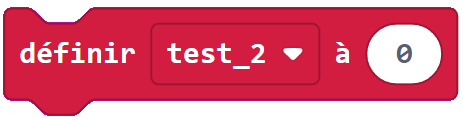
\includegraphics[scale=.5]{ch6_images/var_1}
\end{center}
\item En Python, une variable est créée lorsqu'on lui assigne une valeur.

\vskip.5cm
\begin{lstlisting}[language=python]
variable = 5
nombre_eleve = 16
\end{lstlisting}

\end{enumerate}
\end{remarques}
	
	
	

	
	
	
\begin{exercice}
 Regarder le programme suivant, et deviner ce qu'il va se passer quand on va activer le Microbit:

\begin{center}
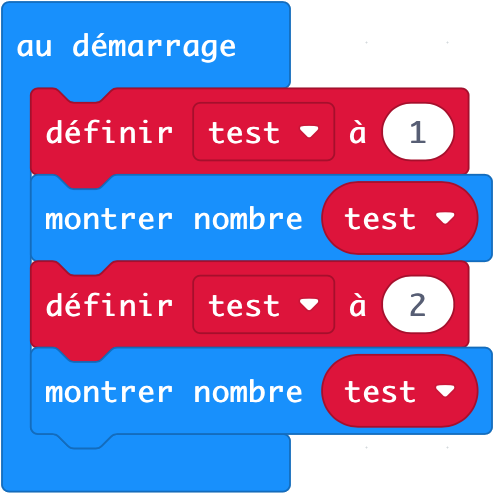
\includegraphics[scale=.6]{ch6_images/var_2}
\end{center}
\end{exercice}


\begin{exercice}
Regarder le programme en python suivant et deviner ce qu'il va se passer quand on va l'exécuter:
\vskip.5cm
\begin{center}
\begin{lstlisting}[language=python]
eleve=20
enseignant=2
print(eleve)
print(enseignant)
    
\end{lstlisting}
\end{center}
\end{exercice}




\subsection{Nom d'une variable}
% Edoardo (14.11.2021)
Le nom choisi pour chaque variable est important pour faciliter la lisibilité de votre programme. Il vous permet de vous souvenir du rôle de chaque variable. Imaginez des milliers de blocs d'instructions Microbit dans votre programme avec des centaines de variables. Si vous nommez vos variables avec des noms peu explicites comme v1, v2, v3, v4 ... v100 seriez-vous capable de retrouver à quoi sert chaque variable ?

Bien que nous soyons toujours libre d'écrire le nom d'une variable comme bon nous semble, un certain nombre de convention sont utilisées:
\begin{enumerate}[1)]
\item Un nom pertinent : essayez d'être le plus précis et concis possible, mais préférez la compréhension à la longueur du nom de la variable. 
\item Toujours commencer par une minuscule
\item Pas de caractères spéciaux ou d'accents
\item Si une variable est un mot composé, deux solutions s'offrent à vous :
\begin{enumerate}[a)] 
\item Notation {\it camel case} : voiciUnExemple. Chaque nouveau mot commence par une majuscule.
\item  Notation {\it snake case} : voici\_ un\_ exemple. Chaque nouveau mot est séparé par un {\it underscore}:\_.

\end{enumerate}
\end{enumerate}

\begin{exercice}
Parmi les noms de variables suivants, lesquels respectent les conventions d'écritures des variables?
\begin{enumerate}
\item laVariable
\item la variable
\item nom\_de\_famille
\item la\_quantité
\item nombreDeVoitures
\item prenom
\item leNumeroDeTelephone
\item le\_ Nom
\item iztrdr3fsfs

\end{enumerate}
\end{exercice}


\subsection{\'Evolution d'une variable}

\subsubsection{En Microbit}

En Microbit il existe deux façon de modifier une variable. La première consiste à lui attribuer une valeur, comme on l'a vu précédemment, avec le bloc {\it Définir variable à ...}:

\begin{center}
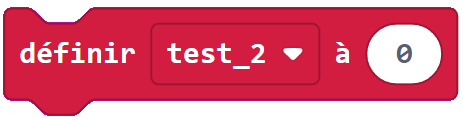
\includegraphics[scale=.4]{ch6_images/var_1}
\end{center}

L'autre façon de modifier une variable consiste à lui ajouter ou soustraire un certain nombre avec le bloc:

\begin{center}
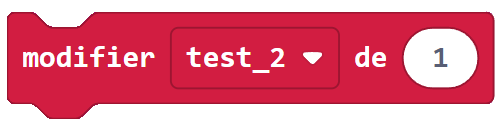
\includegraphics[scale=.4]{ch6_images/var_3}
\end{center}

On peut dire qu'on {\bf incrémente} la variable {\it test\_2}. {\bf Incrémenter} signifie ajouter une certaine valeur, souvent 1, à un nombre ou une variable. Dans le bloc précédent, la valeur de {\it test\_2} va changer et son contenu passera de 0 à 1. 

On parler de {\bf décrémenter} quand on soustrait une certaine valeur. Par exemple, dans le bloc suivant la variable {\it test\_2} qui valait 1, voit son contenu passer de 1 à 0.

\begin{center}

\includegraphics[scale=.4]{ch6_images/var_3a}
\end{center}

Il est aussi possible de mettre un calcul dans l'attribution d'une valeur à la variable. Le prochain bloc d'instruction définit la valeur de la variable {\it var\_1} au résultat du calcul $2+4$.

\begin{center}
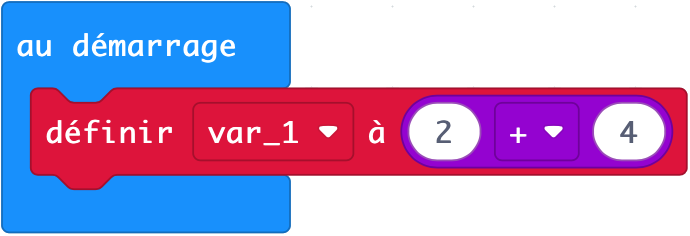
\includegraphics[scale=.5]{ch6_images/var_5}
\end{center}

Ou même d'utiliser la valeur de la variable elle-même:

\begin{center}
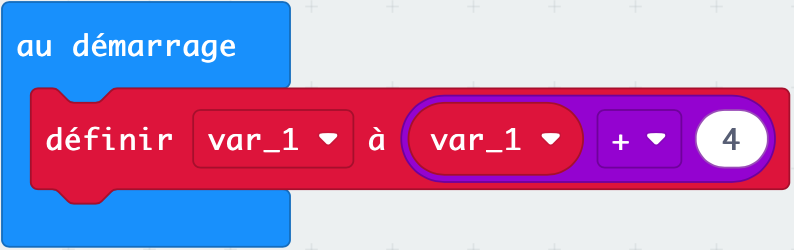
\includegraphics[scale=.5]{ch6_images/var_6}
\end{center}
Dans ce cas de figure, on additionne 4 au contenu de la {\it var\_1}. La variable {\it var\_1} verra ainsi sa valeur actuelle incrémentée de 4.

\subsubsection{En Python}

En Python, pour donner une valeur à une variable, nous allons utiliser le signe "=":

\vskip.5cm
\begin{lstlisting}
classe=16
\end{lstlisting}

Pour incrémenter une variable nous allons écrire:

\vskip.5cm
\begin{lstlisting}
classe=classe+1
\end{lstlisting}

Cette écriture peut prêter à confusion:

\begin{enumerate}
\item Elle n'a pas de sens mathématique.
\item Le signe "=" n'a donc pas la même signification en informatique et en mathématique!
\item Il s’agit d’un symbole d’affectation (nous plaçons un certain contenu dans une variable) et non un symbole d’égalité.
\item Il faut le lire comme: {\it la variable classe prend comme nouvelle valeur son ancienne valeur à laquelle on ajoute 4.} 
\end{enumerate}


Il est donc très important de comprendre cette finesse liée à la programmation !

\subsection*{Exercices}

\begin{exercice}
Quel nombre sera affiché par le programme?
\begin{center}
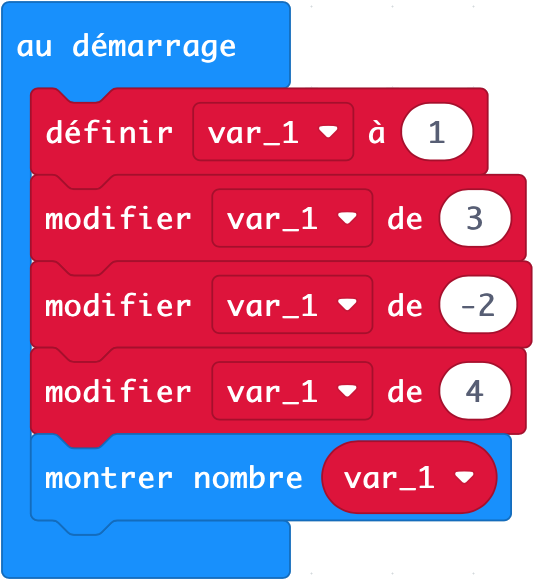
\includegraphics[scale=.5]{ch6_images/var_4}
\end{center}
\end{exercice}

\begin{exercice}
Quel nombre sera affiché par le programme?
\begin{center}
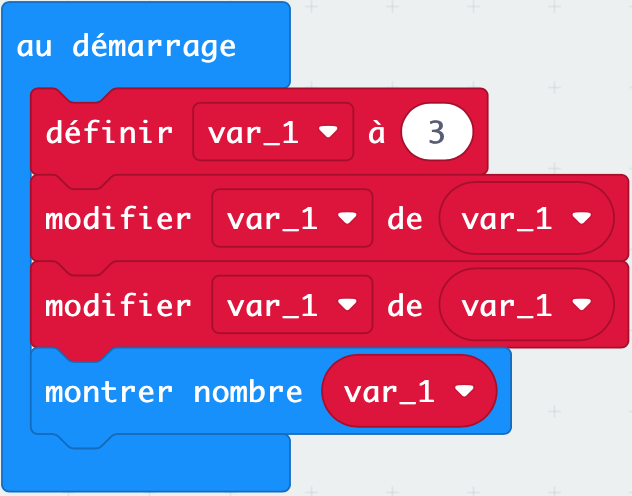
\includegraphics[scale=.5]{ch6_images/var_7}
\end{center}
\end{exercice}

\begin{exercice}
Quel nombre sera affiché par le programme?
\begin{center}
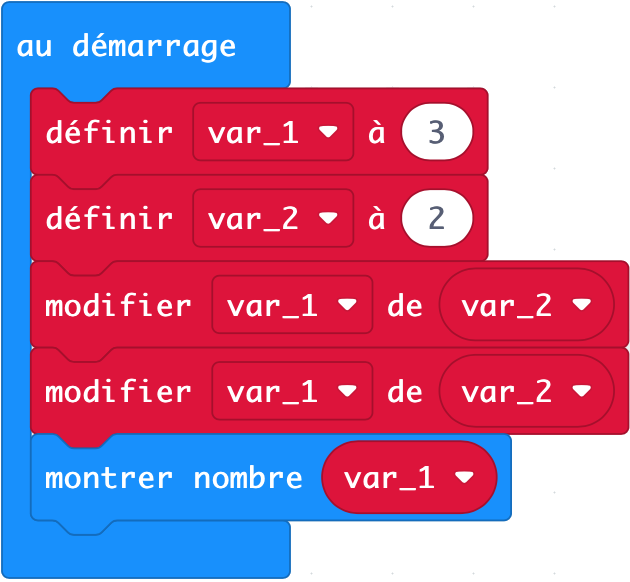
\includegraphics[scale=.5]{ch6_images/var_8}
\end{center}
\end{exercice}



\begin{exercice}
Quels nombres seront affichés par le programme?
\begin{center}
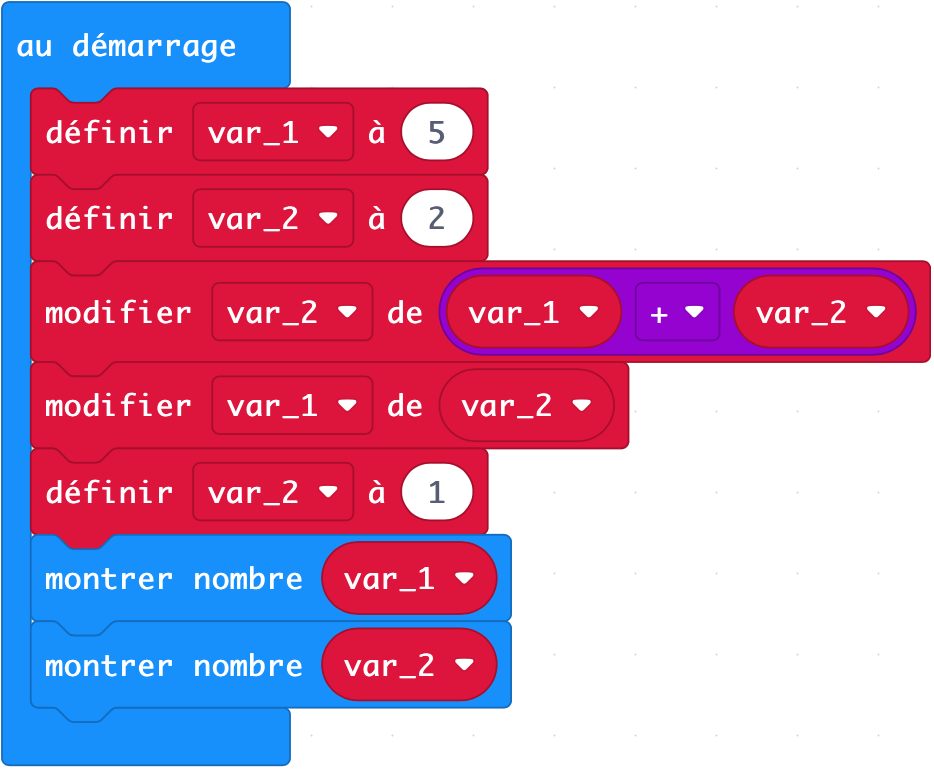
\includegraphics[scale=.5]{ch6_images/var_9}
\end{center}
\end{exercice}


\begin{exercice}
Que fait ce programme?

\vskip.5cm
\begin{lstlisting}
argent=10
argent=argent+5
argent=argent-3
argent=argent*2
print(argent)
\end{lstlisting}
\end{exercice}


\begin{exercice}
Que fait ce programme?

\vskip.5cm
\begin{lstlisting}
benefice=12
benefice=benefice+benefice
benefice=benefice-benefice
print(benefice)
\end{lstlisting}
\end{exercice}

\begin{exercice}
Que fait ce programme?

\vskip.5cm
\begin{lstlisting}
benefice = 12
perte = -3
benefice = benefice + perte
perte = perte + benefice
benefice = benefice + benefice
print(benefice)
print(perte)
\end{lstlisting}
\end{exercice}



\begin{exercice}
Que fait ce programme?

\vskip.5cm
\begin{lstlisting}
premier = 15
deuxieme = 10
difference = premier - deuxieme
deuxieme = premier + difference
premier = difference - deuxieme
difference = deuxieme - premier
print(premier)
print(deuxieme)
print(difference)
\end{lstlisting}
\end{exercice}



\section{Les types}

\subsection{Motivation}

\subsubsection{En Microbit}

Une variable n'aura pas toujours comme valeur un nombre. Dans l'onglet {\it Avancé} ensuite {\it Texte} de l'éditeur makecode.microbit.org, il est possible de choisir le symbole " " représentant une chaîne de caractères. Ainsi il est possible d'attribuer comme valeur une chaîne de caractères: 

\begin{center}
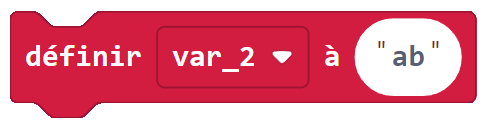
\includegraphics[scale=.4]{ch6_images/var_10}
\end{center}

Ainsi la variable {\it var\_2} est une chaîne de caractères. Essayons d'imaginer ce qu'il va se passer si nous faisons le programme suivant:

\begin{center}
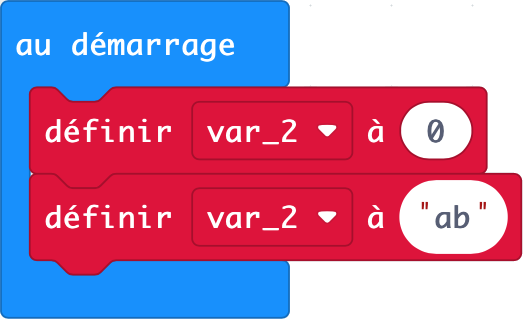
\includegraphics[scale=.5]{ch6_images/var_11}
\end{center}

Que se passe-t-il?

\vskip4cm

Lorsque Microbit repère un problème, il le signale. Dans l'exercice qui suit, essayez de comprendre le problème qui a été rencontré:

\begin{exercice}
Quel problème a été rencontré dans chacun de ces programmes?

\begin{center}
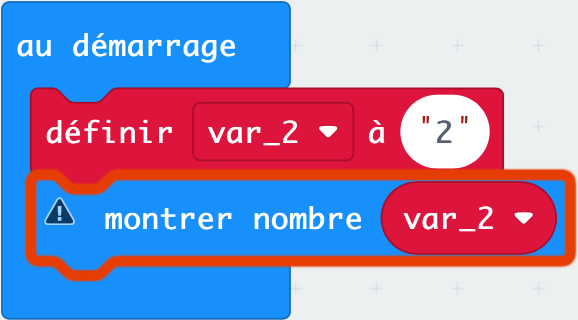
\includegraphics[scale=.5]{ch6_images/var_12}
\end{center}

\begin{center}
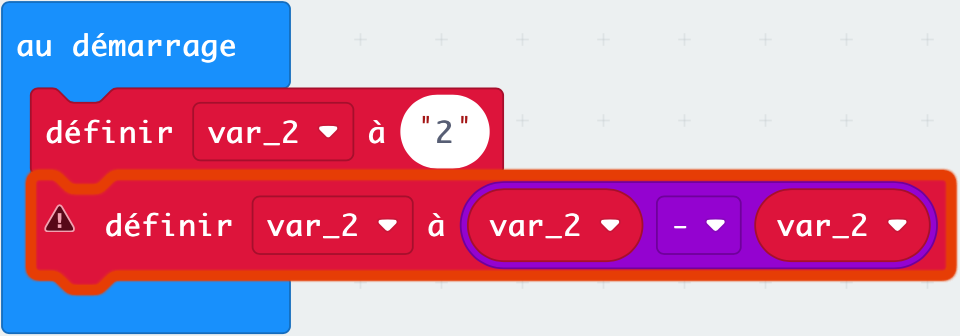
\includegraphics[scale=.5]{ch6_images/var_13}
\end{center}

\end{exercice}

\begin{remarque}
Chaque langage de programmation aura ses propres spécificités par rapport aux différents types d'erreurs qui peuvent apparaître. Par exemple, en Microbit, le programme ci-dessous fonctionne, et affiche 22!!

\begin{center}
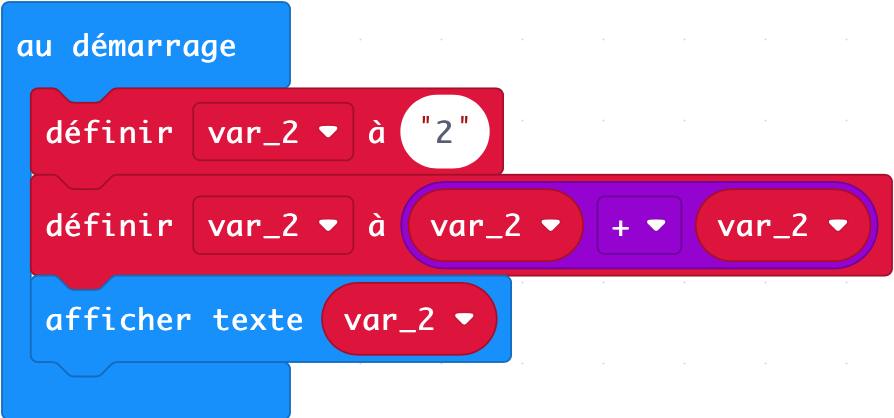
\includegraphics[scale=.5]{ch6_images/var_14}
\end{center}
\end{remarque}

\subsubsection{En Python}

En Python, contrairement à Microbit, une variable peut d'abord valoir un nombre puis ensuite un caractère ou un mot. 


\vskip.5cm
\begin{lstlisting}
a=2
print(a)
a="bonjour"
print(a)
\end{lstlisting}
\vskip.5cm

Le programme précédent afficher d'abord le nombre 2 puis le mot "bonjour". 

\begin{exercice}
A votre avis, que fait le programme suivant?

{\it (indication: le programme fonctionne})

\vskip.5cm
\begin{lstlisting}
a=5
b="2"
d=2
c=a*d
print(c)
c=a*b
print(c)
\end{lstlisting}
\end{exercice}
\vskip.5cm

\subsection{Définition}

On a vu que suivant la valeur attribuée à une variable, le programme va permettre de faire certaines actions et en refuser d'autre. On définit cela formellement:

\begin{defi}
Le {\it type} d'une variable est l'interprétation que fera l'ordinateur de la valeur associée à cette variable. Ce type pourra être, entre autre, un nombre entier ({\it integer}), un nombre décimal ({\it float}), une chaîne de caractère ({\it string}), un booléen ({\it boolean})...
\end{defi}

Selon le langage de programmation que l'on utilise, le type d'une variable peut ou ne peut pas être changé. On parlera de {\bf typage statique} ou {\bf typage dynamique}. Par exemple, Microbit a un typage statique (Une variable définit comme un nombre ne peut plus être changé en une chaîne de caractères) alors que Python a un typage dynamique. 

On regarde maintenant chacun de ces types en détail. 



\subsection{Les types {\it entier} (integer) et {\it décimal} (float)}

La première catégorie de variables avec laquelle on aimerait travailler est le nombre. Cette catégorie se divise en 2 catégories principales. Comme nous l'avons vu, un nombre entier (positif ou négatif) n'utilise pas le même encodage qu'un nombre à virgule (qui utilise plutôt un encodage sous la forme d'une écriture scientifique). L'espace mémoire n'est donc pas le même. 

\begin{defi}
Le type {\it entier} (integer) caractérise une variable dont la valeur est un nombre entier. Le type {\it décimal} (float) caractérise une variable dont la valeur est un nombre décimal.
\end{defi}

Pour un programme, {\bf 1} sera un {\it entier} alors que {\bf 1.0} sera un {\it décimal}.

Pour Microbit ou Python, ainsi que pour de nombreux langages de programmation, il n'y a pas de problèmes à passer d'un nombre entier à un nombre décimal au cours du programme sans devoir changer de variable et de type.


\subsection{Le type {\it chaîne de caractères} (string)}

Une autre valeur que peut prendre une variable est la chaîne de caractères, ou le type {\it string}.

\begin{defi}
Le type {\it chaîne de caractères} (string) caractérise une variable dont la valeur est une suite de caractères. Cette suite peut aussi contenir des nombres qui sont alors interprétés comme des caractères.
\end{defi}

Le programme suivant n'a par exemple aucune signification pour Microbit:

\begin{center}
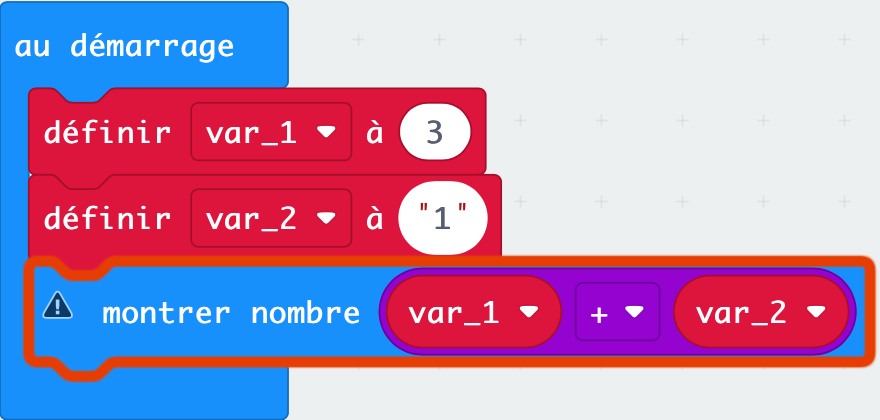
\includegraphics[scale=.5]{ch6_images/var_15}
\end{center}

Le même problème apparait en Python. Un message d'erreur nous dira que nous ne pouvons pas faire "+" entre un "int" et un "str":

\vskip.5cm
\begin{lstlisting}
a=5
b="2"
c=a+b
\end{lstlisting}
\vskip.5cm


Nous ne pouvons pas effectuer d'opération avec les chaînes des caractères (sauf le + que l'on verra par la suite). Il est par contre possible de comparer des chaînes de caractères:

\begin{center}
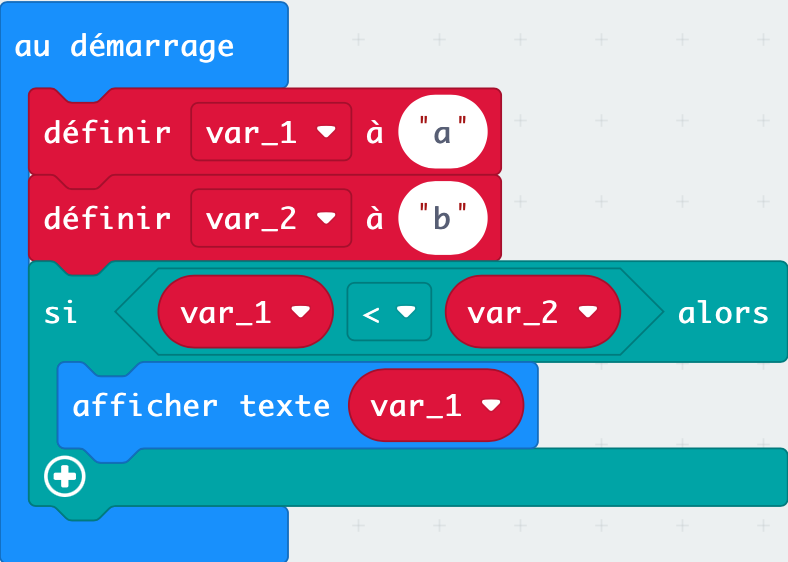
\includegraphics[scale=.5]{ch6_images/var_16}
\end{center}
Dans ce cas, comme la lettre a (contenu dans {\it var\_1}) se trouve avant b (contenu dans ({\it var\_2}) en prenant compte de l'ordre alphabétique, le texte contenu dans la {\it var\_1} s'affiche. Le Microbit affiche le texte a.

% Edoardo, 17.11.2021
Prenons un autre exemple:
\begin{center}
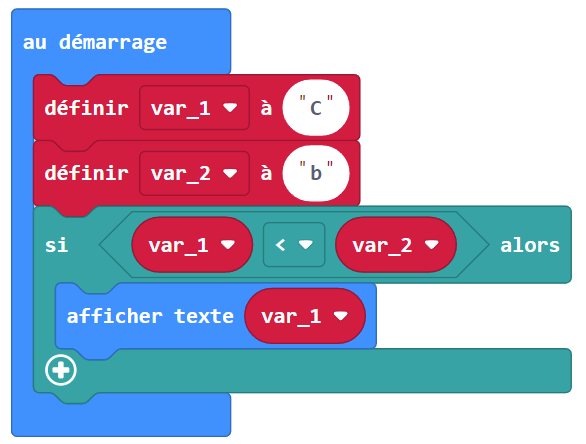
\includegraphics[scale=.5]{ch6_images/var_16a}
\end{center}
Dans ce cas, Microbit affiche C. Pourquoi le programme considère t'il que C est plus petit que b ? Tout simplement parce qu'il se base sur son code ASCII pour comparer ! Le code ASCII de C est 67 (base 10) alors que b est 98 (base 10).
% end Edoardo

\newline

L'opération principale sur les chaînes de caractères est la {\bf concaténation}:

\begin{defi}
La {\it concaténation} est une action qui prend en entrée plusieurs chaînes de caractères et renvoie une unique chaîne de caractères composée des différentes chaînes de caractères misent bout à bout.
\end{defi}

Par exemple, {\it concaténation("abc"; "d2")="abcd2"}.

\ 

Dans Microbit, l'opération + a le même effet que la concaténation si on lui donne deux chaînes de caractères. Ainsi, le programme suivant donnera "32":

\begin{center}
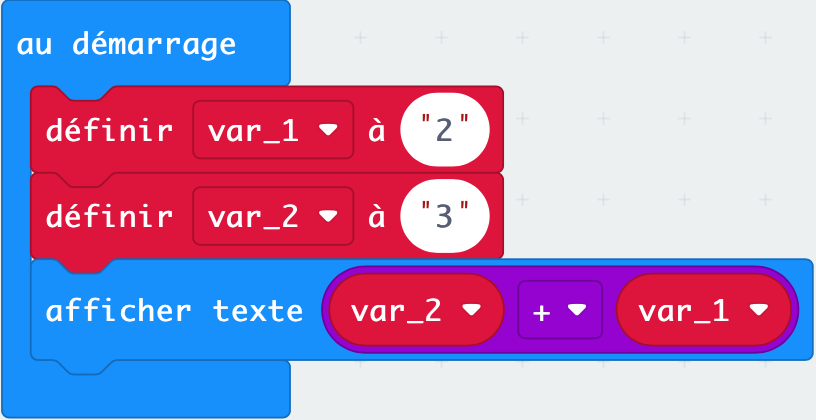
\includegraphics[scale=.5]{ch6_images/var_17}
\end{center}

Alors que le programme ci-dessous va afficher 5:

\begin{center}
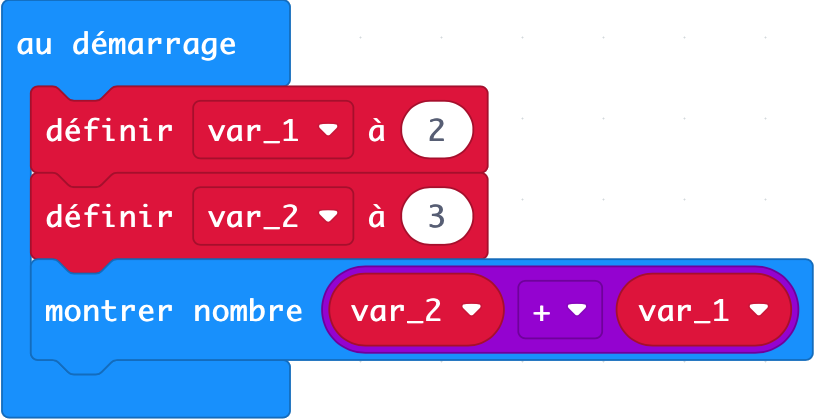
\includegraphics[scale=.5]{ch6_images/var_18}
\end{center}

En Python, la concaténation passe par le +. Le programme suivant affichera "5d":

\vskip.5cm
\begin{lstlisting}
a="5"
b="d"
c=a+b
print(c)
\end{lstlisting}
\vskip.5cm

\subsubsection{Affichage d'une variable}

Les guillemets précisent qu'on a à faire à une chaine de caractères. Cette différence est importante comme on peut le noter dans le programme suivant:

\vskip.5cm
\begin{lstlisting}
test=25
print(test)
print("test")
\end{lstlisting}
\vskip.5cm

Ce programme afficher d'abord la variable test, donc 25. Puis affichera le texte "test". 

\subsection{Le type {\it booléen} (boolean)} 

En informatique nous devons souvent tester une condition ("le nombre suivant est il pair?", "la variable vaut-elle 2?"...). Pour cela, nous avons besoin d'un type de variable qui ne correspondra ni à un nombre ni à une chaîne de caractères mais qui pourra nous permettre de résoudre un problème du type: si "il pleut", alors "il faut prendre un parapluie". Le test "il pleut" peut prendre deux valeurs: soit c'est vrai, soit c'est faux. C'est ce que nous appelons une {\bf variable booléenne}:

\begin{defi}
Le type {\it booléen} caractérise une variable qui peut avoir une des deux valeurs suivantes: "vrai" ou "faux".
\end{defi}

\subsubsection{En Microbit}
% Edoardo 27.11.2021
Dans Microbit, le type booléen est noté par un hexagone vert. Dans le cas suivant la variable {\it var\_1} est initialisée avec la valeur vrai ({\it true}).
\begin{center}
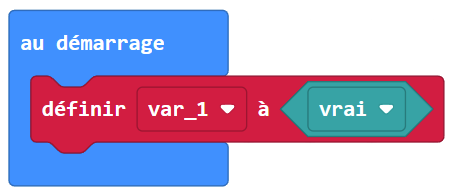
\includegraphics[scale=.5]{ch6_images/var_19a}
\end{center}
% End Edoardo

On remarque qu'une variable booléenne ne peut pas être affichée comme un nombre dans Microbit:

\begin{center}
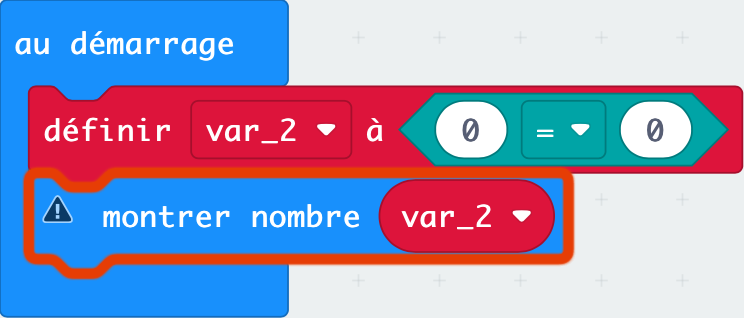
\includegraphics[scale=.5]{ch6_images/var_19}
\end{center}

Mais il peut être affiché comme un texte (le Microbit affiche {\it true} même si votre éditeur de code est configuré en français):

\begin{center}
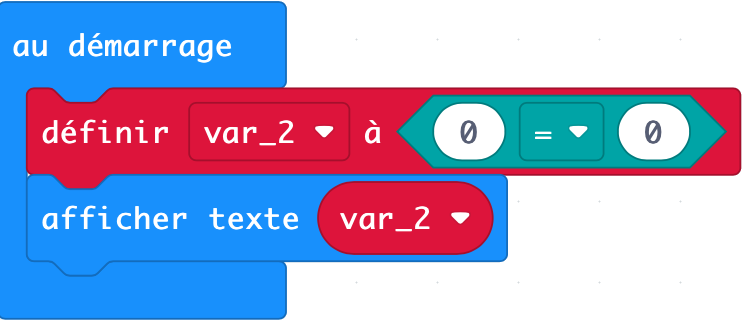
\includegraphics[scale=.5]{ch6_images/var_20}
\end{center}


\subsubsection{En python}

En Python, un booléen va souvent être sous la forme d'une comparaison ou d'une égalité. On voudra par exemple vérifier que l'âge de quelqu'un est strictement inférieur à 12 ans pour avoir une réduction:

\vskip.5cm
\begin{lstlisting}
if age < 12:
    print("Vous avez le droit à une réduction")
\end{lstlisting}
\vskip.5cm

"age<12" est un booléen, c'est soit vrai, soit faux. Si c'est vrai, alors on affichera "Vous avez le droit à une réduction". Et si c'est faux, rien ne sera fait. 

D'autres comparaisons peuvent être faites:

\begin{enumerate}
    \item l'égalité (attention au double "=" qui montre que l'on vérifie si il y a égalité. le symbole "=" seul est gardé pour assigner une valeur à une variable):
    \vskip.5cm
\begin{lstlisting}
if age == 12:
    print("Vous avez 12 ans.")
\end{lstlisting}
    \vskip.5cm
    \item la différence:
    \vskip.5cm
\begin{lstlisting}
if age != 12:
    print("Vous n'avez pas 12 ans.")
\end{lstlisting}
    \vskip.5cm
    \item plus petit ou égal:
    \vskip.5cm
\begin{lstlisting}
if age <= 12:
    print("Vous avez 12 ans ou moins.")
\end{lstlisting}
    \vskip.5cm
\end{enumerate}




\subsection{Le type {\it liste} (list)}

On peut avoir besoin de rassembler en une même variable un ensemble d'éléments: par exemple les noms des élèves d'une classe, ou les cartes d'un jeu de cartes. Pour cela, il existe un type qui est la {\it liste}:

\begin{defi}
Le type {\it liste} caractérise une variable qui contient une série d'éléments qui peuvent être ou ne pas être du même type (cela dépend du langage de programmation).
\end{defi}

En Python, les éléments d'une liste ne sont pas forcément du même type et un élément d'une liste peut aussi être une liste. Pour créer une liste contenant les éléments 1,2 et 3 nous écrirons:

\vskip.5cm
\begin{lstlisting}
lst = [1,2,3]
\end{lstlisting}
\vskip.5cm

Une liste peut être affiché avec la commande: print(lst). On peut rajouter un élément à une liste en l'additionnant (comme pour une concaténation) à la liste existante. Si par exemple nous voulons rajouter le 4 dans notre liste, nous écrirons:

\vskip.5cm
\begin{lstlisting}
lst = lst + [4]
\end{lstlisting}
\vskip.5cm

Si nous voulons accéder à un élément d'une liste, nous indiquons l'indice de l'élément recherché:
\begin{itemize}
\item lst[0] correspond au premier élément de la liste lst, qui ici est 1.
\item lst[1] correspond au deuxième élément de la liste lst, qui ici est 2... et ainsi de suite.
\end{itemize}


\subsection*{Exercices}

\begin{exercice}
Définir quel type (entier, décimal, chaîne de caractères, booléen,liste) devrait-on associer à une variable si cette variable représente:
\begin{enumerate}[a)]
\item l'âge d'une personne;
\item si il pleut;
\item les prénoms des enfants d'une famille;
\item un mois de l'année;
\item le prix d'un vêtement;
\item si une personne est majeure;
\item une année de naissance;
\item les sports pratiqués par un élève;
\item l'aire d'une forme géométrique;
\item le nom d'une personne;
\item si un végétal donné est un fruit;
\end{enumerate}
\end{exercice}



\begin{exercice}
Donner le type de chaque variable de ce programme puis dire si des erreurs vont être reconnues par Microbit (tester le programme si besoin):
\begin{center}
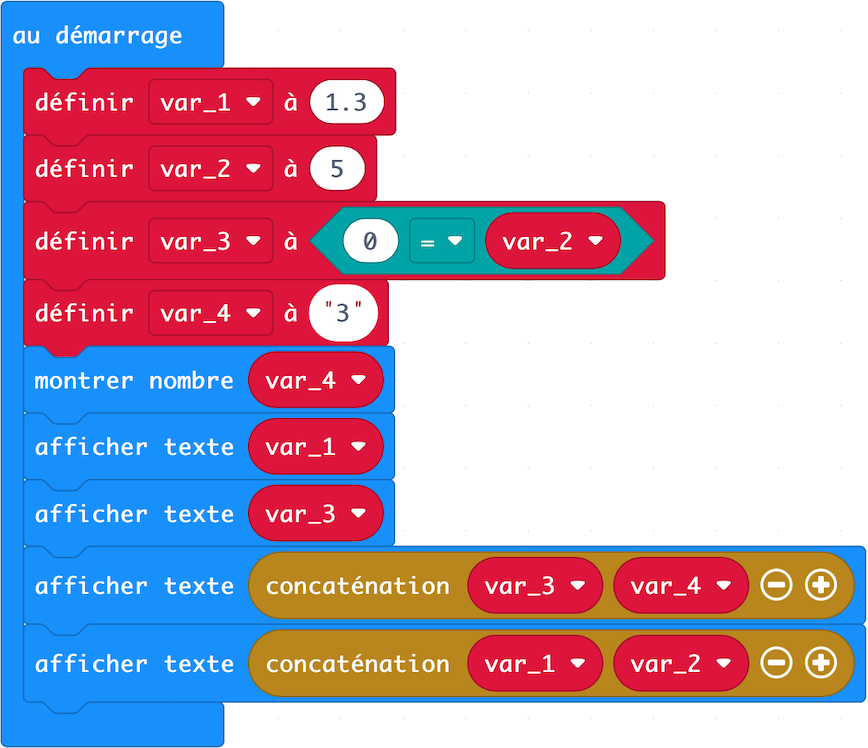
\includegraphics[scale=.7]{ch6_images/var_21}
\end{center}
\end{exercice}


\begin{exercice}
Reconnaître les différents types apparaissant dans ce programme:
\vskip.5cm
\begin{lstlisting}
pi = 3.14
rayon = 5
petit_et_grand = [40,100]
circonference = pi*2*rayon
reponse = "C'est un petit cercle"
if circonference < petit_et_grand[0]:
    print(reponse)
\end{lstlisting}
\vskip.5cm
\end{exercice}

\begin{exercice}
Dire ce qui va être affiché pour chacun des programmes suivants:
\begin{enumerate}

\item 
\vskip.5cm
\begin{lstlisting}
x = 5
y = 12
print(x)
print("y")
print(x < y)
\end{lstlisting}
\vskip.5cm

\item 
\vskip.5cm
\begin{lstlisting}
x = 12
y = 2 * x
print(x == 2 * y)
print(y == 2 * x)
\end{lstlisting}
\vskip.5cm

\end{enumerate}
\end{exercice}


\section{Bases de l'algorithmique}

Nous allons commencer à discuter ce que représente un algorithme et comment peut-on décomposer une tâche en tâches plus élémentaires dans le but de résoudre un problème ou d'accomplir un travail. La pensée algorithmique est un pan essentiel de l'informatique. Une fois correctement formulée ou précisée, elle permet, via un langage de programmation, d'implémenter différents traitements sur les machines (par exemple votre ordinateur).


\subsection{Définition}
\begin{defi}
Un algorithme est une suite finie et non-ambiguë d'opérations ou d'instructions permettant de résoudre un problème.

\end{defi}

On connaît depuis l'antiquité des algorithmes sur les nombres, comme par exemple l'algorithme d'Euclide qui permet de calculer le {\it pgdc}\footnote{pgdc: plus grand diviseur commun.} de deux nombres entiers.

Pour le traitement de l'information, on a développé des algorithmes opérant sur des données non numériques : les algorithmes de tri, qui permettent par exemple de ranger par ordre alphabétique une suite de noms, les algorithmes de recherche d'une chaîne de caractères dans un texte, ou les algorithmes d'ordonnancement, qui permettent de décrire la coordination entre différentes tâches, nécessaire pour mener à bien un projet.

Algorithme provient du nom du mathématicien perse {\it  Al-Khawarizmi} ($\sim$ 820), le père de l'algèbre.

\subsection{Les structures de contrôle}

Pour construire un algorithme, nous avons besoin d'une suite d'instructions. Ces instructions sont prises parmi un ensemble de {\it fonctions} pour Python  ou de {\it blocs} pour Microbit et sont exécutées les unes après les autres. Afin de {\it répéter} une même action un certain nombre de fois ou de faire une action {\it si} une condition est vraie, nous avons besoin de structure de contrôle:

\begin{defi}
Une {\it structure de contrôle } détermine dans quel ordre vont être exécutées les actions. Il en existe trois:
\begin{enumerate}
\item La {\it séquence}: les instructions sont effectuées les unes après les autres
\item La {\it sélection}: les instructions sont effectuées si une certaine
 condition est respectée (par exemple la structure {\it si})
\item La {\it répétition}: les instructions sont répétées en boucle {\it tant qu}'une certaine condition est respectée.
\end{enumerate}
\end{defi}

Ses structures sont récurrentes et apparaissent toujours sous une forme ou sous une autre dans presque tous les langages de programmation. Nous allons maintenant étudier les différentes structures qui sont à notre disposition.

\subsection{La condition {\it si} (if)}

\subsubsection{le {\it if} simple}

Une des premières structures qui nous intéresse est la structure de sélection {\it si} ou {\it if} en anglais. Sa syntaxe en pseudo-code est de la forme:

\ 

\hskip5cm {\it si} {\bf condition} 
	
\hskip+6cm alors {\bf action}

\ 

Le {\it si} vérifie si la {\bf condition} est {\it vraie} et si c'est le cas, la ligne avec l'{\bf action} est effectuée. La {\bf condition} est donc forcément un {\bf booléen} qui sera soit vrai soit faux.

Par exemple, on peut avoir le code suivant:

\ 

\hskip5cm {\it si} {\bf il pleut} 
	
\hskip+6cm alors {\bf je prends mon parapluie}

\ 

{\bf il pleut} est bien un booléen. Cela est soit vrai soit faux. Si cela est vrai, la ligne {\bf je prends mon parapluie} est exécutée. Si c'est faux, cette ligne ne sera pas évaluée. 

Pour un code Microbit, cela donnerait:

\begin{center}
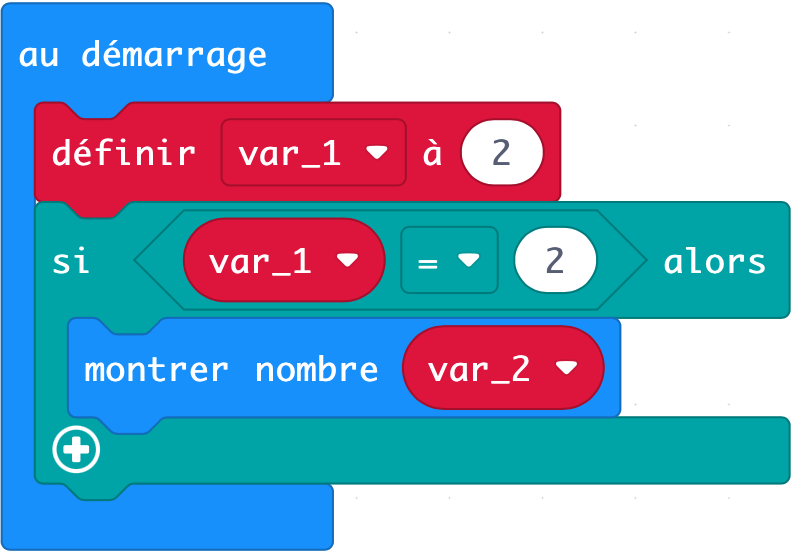
\includegraphics[scale=.45]{ch6_images/var_22}
\end{center}

En Python, l'expression d'une condition commence par un {\bf if}, suivi d'un booléen puis de deux points ":". Tout ce qu'il faudra faire si la condition est vérifiée doit être indenté:

\vskip.5cm
\begin{lstlisting}
variable=1
if variable == 2:
    print(variable)   
\end{lstlisting}
\vskip.5cm

L'indentation est très importante. Pour le comprendre, voici trois exemple et ce qu'ils affichent:

\vskip.5cm
\begin{lstlisting}
variable=1
if variable == 2:
    print(variable)
    print("fin")
\end{lstlisting}
\vskip.5cm

Dans ce programme, rien n'est fait. La condition n'est pas vérifiée, donc les instructions incluses dans le {\bf if} (celles avec une indentation) ne sont pas effectuées.

\vskip.5cm
\begin{lstlisting}
variable=1
if variable == 2:
    print(variable)
print("fin")
\end{lstlisting}
\vskip.5cm

Dans ce programme, "fin" est affiché. La condition du {\bf if} n'est pas vérifiée et donc l'instruction "print(variable)" n'est pas faite. Par contre, en retournant à la ligne par la suite, on indique que nous sortons du {\bf if} et l'instruction "print("fin")" est effectué.

\subsubsection{Multiples conditions}


Une condition {\it si} peut vérifier d'autres conditions, qui débutent par {\it sinon si} (else, if) et peut aussi finir par un {\it sinon} (else) qui ne sera exécuté que si toutes les autres conditions étaient fausses:


\hskip+5cm {\it Si} {\bf j'ai entre 500 et 1000 .-} 
	
\hskip+6cm alors {\bf je pars en Europe}

\hskip+5cm {\it sinon, si} {\bf j'ai entre 1000 et 2000 .-} 
	
\hskip+6cm alors {\bf je pars en Asie}

\hskip+5cm {\it sinon, si} {\bf j'ai plus que 2000.-} 
	
\hskip+6cm alors {\bf je pars en Amérique}

\hskip+5cm {\it sinon}  {\bf je reste chez moi}

\ 

Le programme équivalent en Microbit serait:

\begin{center}
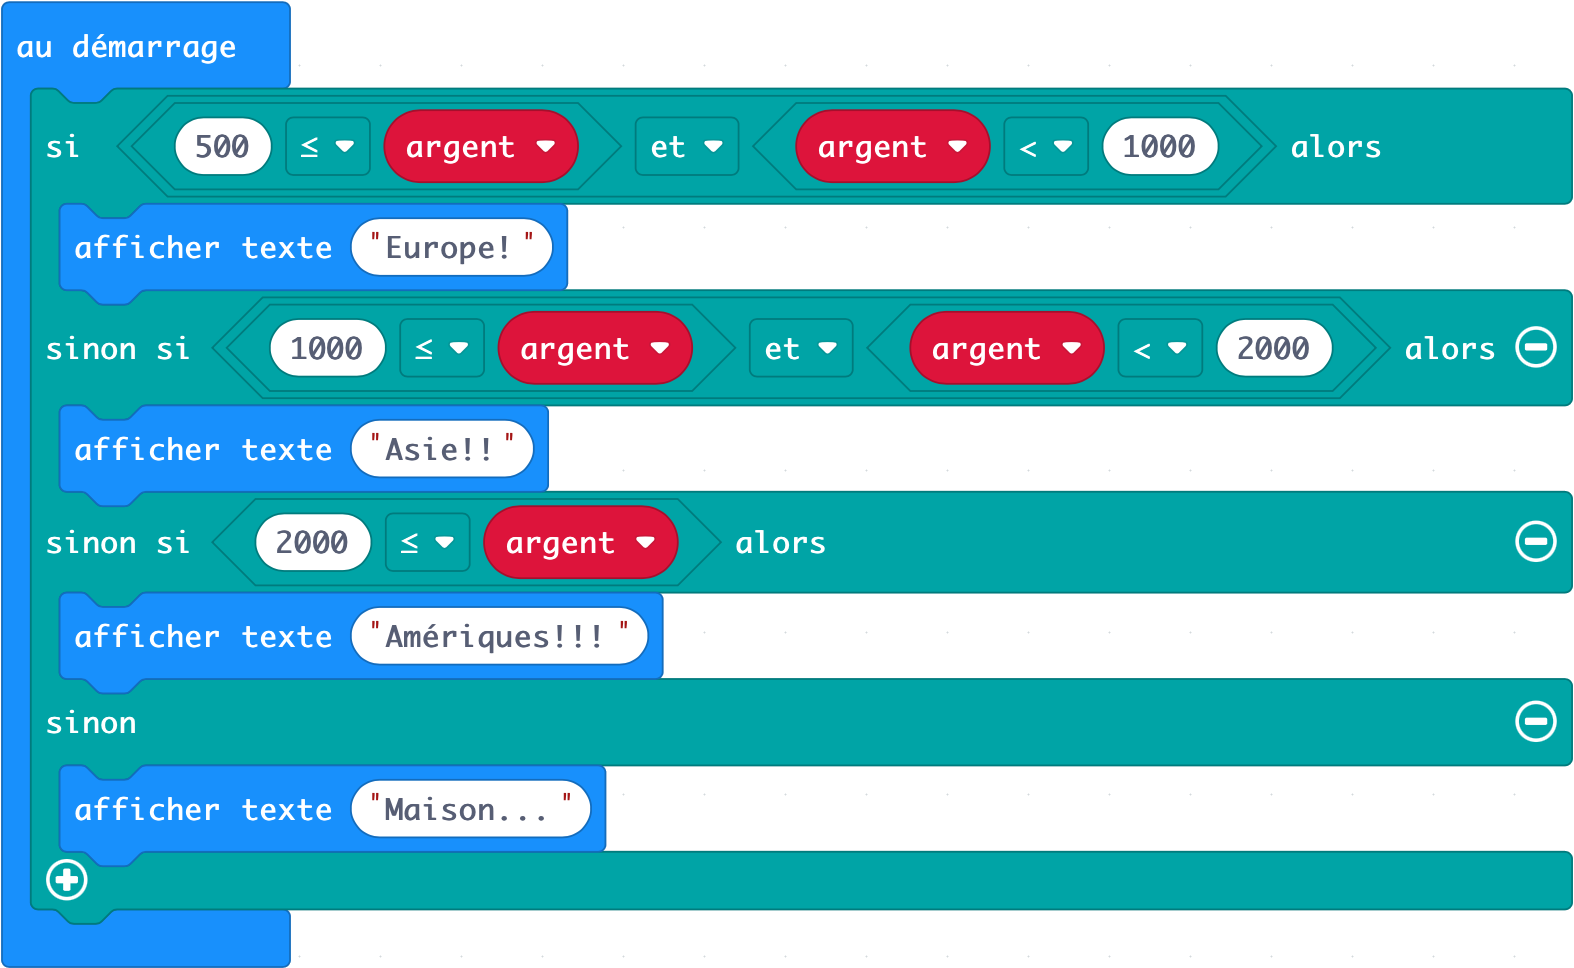
\includegraphics[scale=.4]{ch6_images/var_23}
\end{center}

\

En python, une condition commence par un {\bf if} et est suivi par autant de {\bf elif} (contraction de {\it else, if} (sinon, si)) nécessaire et fini, si besoin, par un {\bf else} (sinon) qui lui ne vérifie aucune condition.

\vskip.5cm
\begin{lstlisting}
if 500 <= argent and argent <= 100 :
    print("Europe")
elif 1000 <= argent and argent <= 2000:
    print("Asie!")
elif 2000 <= argent:
    print("Amerique!!!")
else:
    print("Maison...")
\end{lstlisting}
\vskip.5cm

\subsubsection*{Exercices}


\begin{exercice}
Qu'affiche ce programme?
\begin{center}
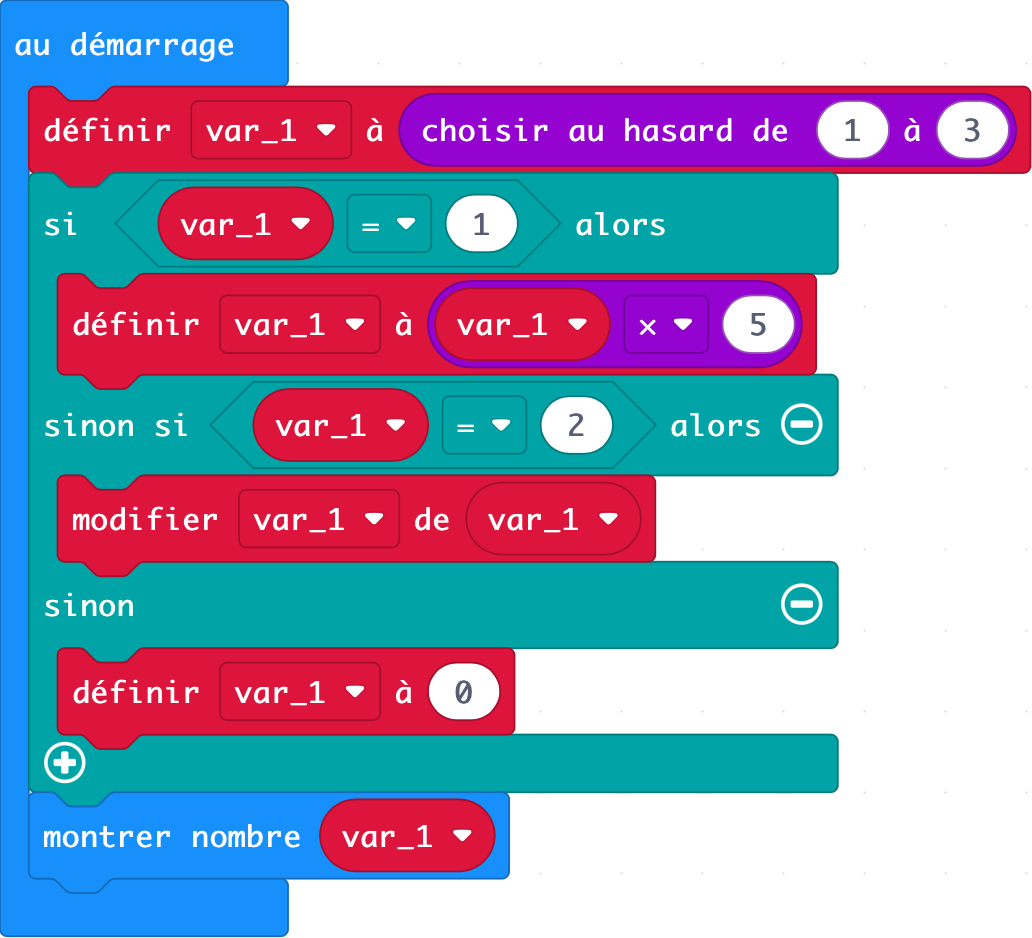
\includegraphics[scale=.4]{ch6_images/var_24}
\end{center}
\end{exercice}

\begin{exercice}
Qu'affiche ce programme?
\begin{center}
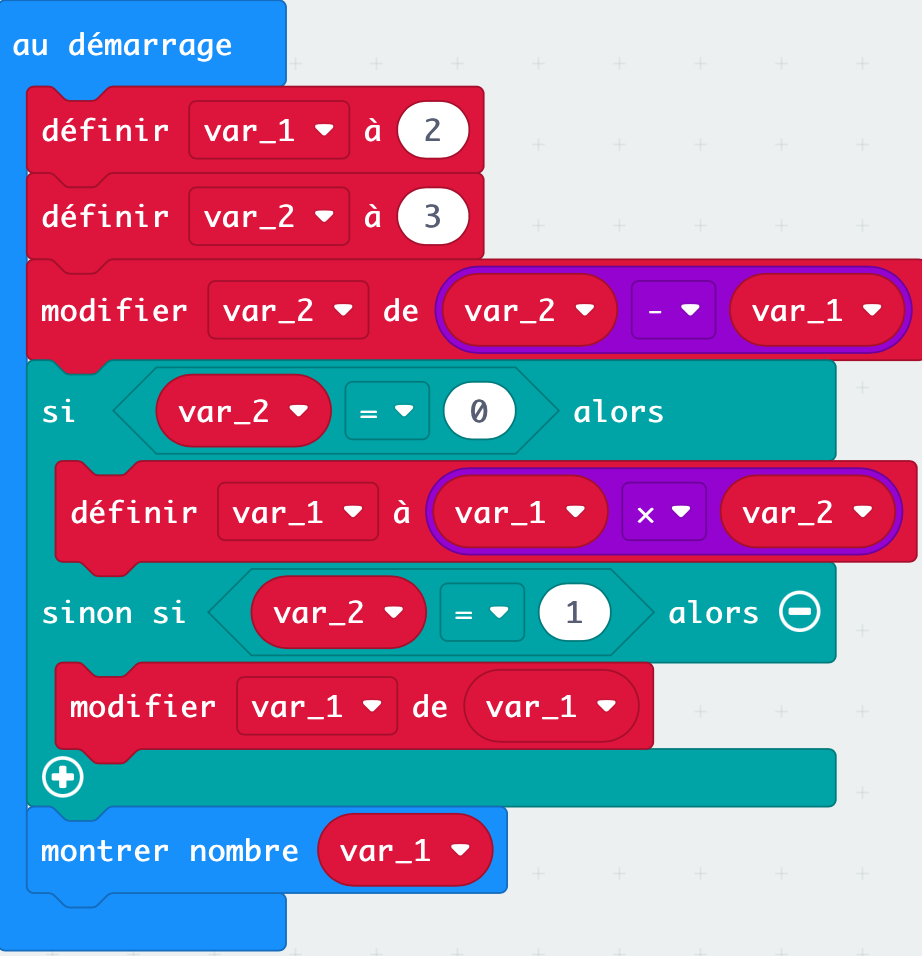
\includegraphics[scale=.4]{ch6_images/var_25}
\end{center}
\end{exercice}

\begin{exercice}
\begin{center}
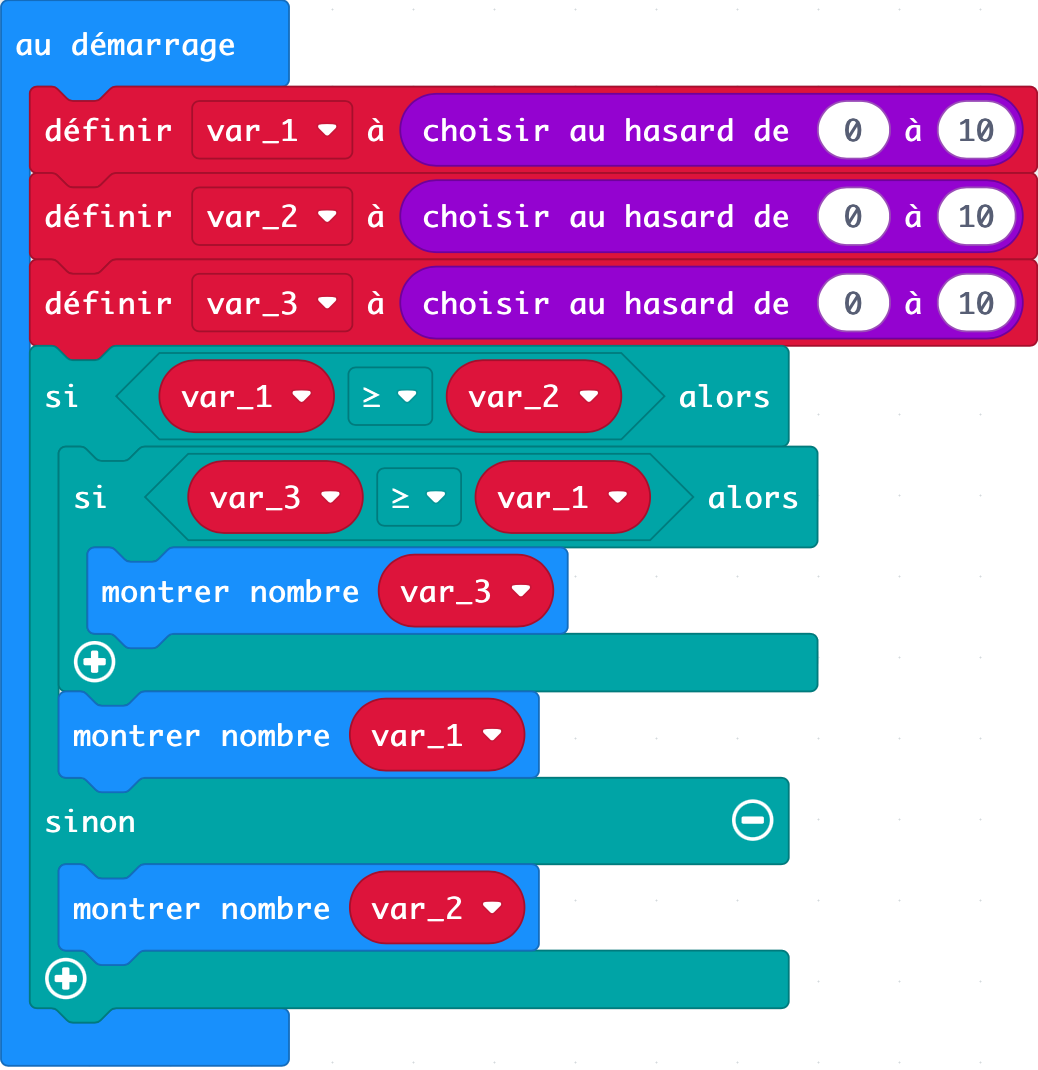
\includegraphics[scale=.4]{ch6_images/var_26}
\end{center}
Dans chacun des cas suivants, dire ce qu'affichera le programme:
\begin{enumerate}
	\item si $var\_1=5$, $var\_2=9$  et $var\_3=2$. 
	\item si $var\_1=7$, $var\_2=3$  et $var\_3=3$.
	\item si $var\_1=3$, $var\_2=5$  et $var\_3=6$. 
	\item si $var\_1=4$, $var\_2=4$  et $var\_3=4$.  
\end{enumerate}
\end{exercice}

\newpage
\begin{exercice}
Qu'affiche le programme suivant:
\vskip.5cm
\begin{lstlisting}
nombre_1 = 3
nombre_2 = 7
nombre_3 = 10
if nombre_1 == nombre_2 :
    print(nombre_1)
elif nombre_2 < nombre_3 :
    print(nombre_2)
elif nombre_3 == 10 :
    print(nombre_3)
if nombre_2 != 7 :
    print(nombre_2)
else :
    print(nombre_3)
\end{lstlisting}
\vskip.5cm
\end{exercice}


\begin{exercice}


\vskip.5cm
\begin{lstlisting}
if x < y :
    if x < z :
        print(z)
    else :
        print(x)
elif x < z :
    if x > y :
        print(y)
    elif y < z :
        print(z)
if z < y :
    print(y)
print(x)
    
\end{lstlisting}
\vskip.5cm
Dans chacun des cas suivants, dire ce qu'affichera le programme:
\begin{enumerate}
	\item  si $x=3$, $y=5$ et $z=1$.
	\item  si $x=3$, $y=5$ et $z=9$.
	\item  si $x=9$, $y=5$ et $z=1$.
	\item  si $x=6$, $y=3$ et $z=4$.
\end{enumerate}

\end{exercice}

\subsection{La boucle {\it répéter} (repeat)}

\subsubsection{En Microbit}

La condition {\it si} est une structure  nous permettant de coder des conditions mais elle n'est pas suffisante. Pour certain problème, nous avons besoin de répéter une certain nombre de fois une action. Le nombre de répétition peut-être connue à l'avance ou ne pas l'être.

Nous aimerions, par exemple, doubler la valeur de $var\_1$ 5 fois de suite. La première possibilité est la suivante:

\begin{center}
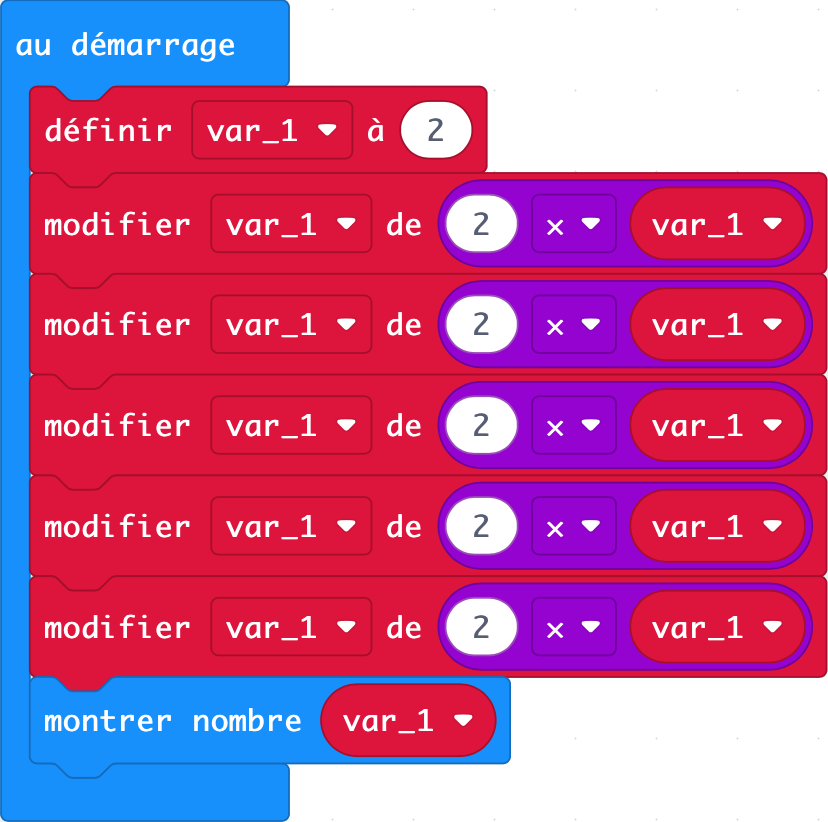
\includegraphics[scale=.5]{ch6_images/var_27}
\end{center}

Lorsque nous répétons plusieurs fois la même action, il est plus facile d'utiliser une boucle {\it répéter} (repeat), qui effectuera une même tâche un certain nombre de fois:

\begin{center}
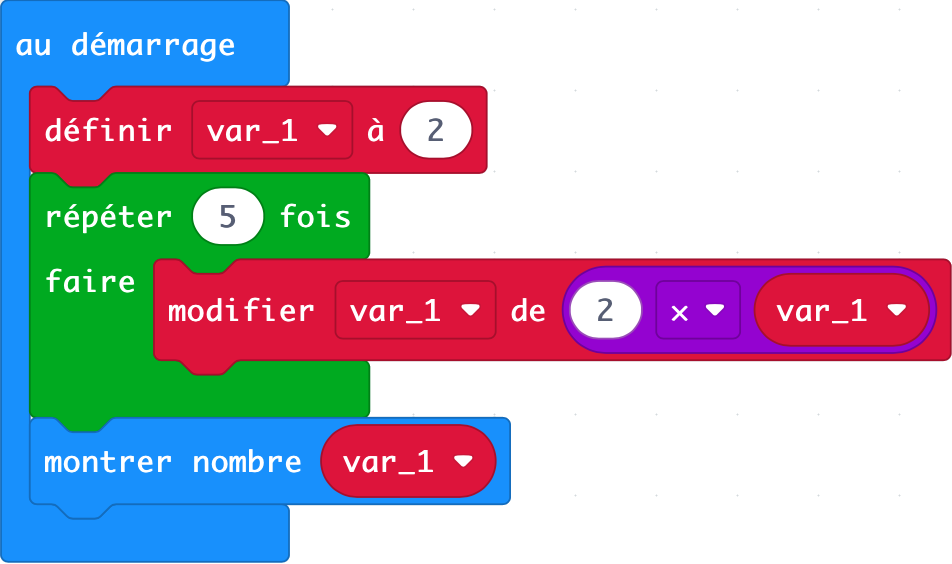
\includegraphics[scale=.5]{ch6_images/var_28}
\end{center}

L'intérêt de {\it répéter} est que nous pouvons aussi utiliser une variable pour le nombre de fois que nous voulons répéter une tâche et donc obtenir une grande flexibilité dans notre programme.

\subsubsection{En Python}

En Python, pour répéter une même tâche on peut utiliser la fonction {\it for}, qui permet de faire de nombreuses choses, dont la répétition. Considérons le programme suivant qui répète plusieurs fois la même tâche:

\vskip.5cm
\begin{lstlisting}
x = 2
x = 2 * x
x = 2 * x
x = 2 * x
x = 2 * x
x = 2 * x
print(x)
\end{lstlisting}
\vskip.5cm

On peut écrire le programme suivant qui effectue la même tâche, mais en moins d'instructions:

\vskip.5cm
\begin{lstlisting}
x = 2
for k in range (5) :
    x = 2 * x
print(x)
\end{lstlisting}
\vskip.5cm

On verra par la suite que la fonction {\it for} permet de faire beaucoup plus qu'une répétition. Dans l'écriture {\it for k in range(5)}, $k$ est une variable et pourrait être nommée avec le nom qu'on souhaite. Il faut par contre éviter de le nommer avec un nom de variable déjà utilisé précédemment.

\subsubsection*{Exercices}


\begin{exercice}
Que fait le programme suivant?
\begin{center}
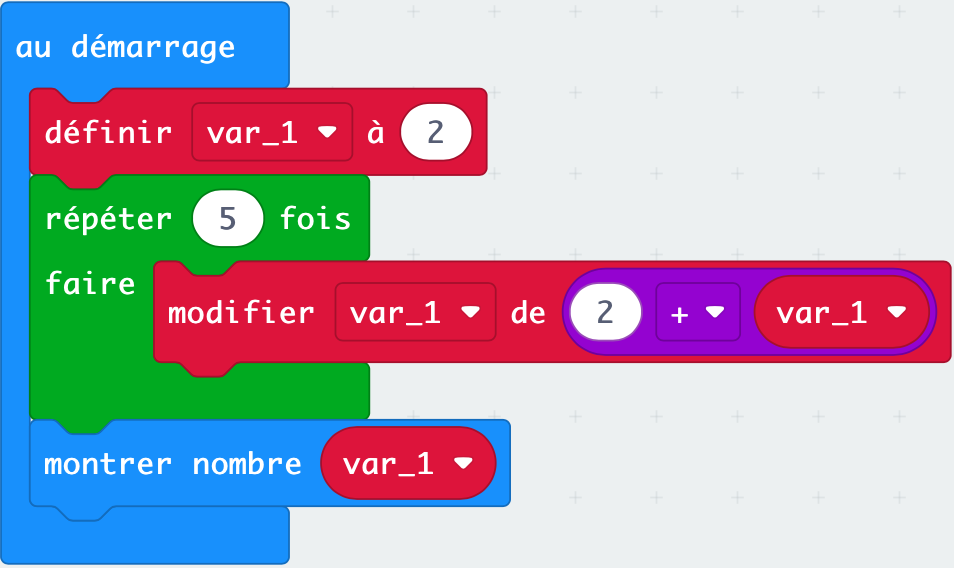
\includegraphics[scale=.5]{ch6_images/var_29}
\end{center}
\end{exercice}


\begin{exercice}
Que fait le programme suivant?
\begin{center}
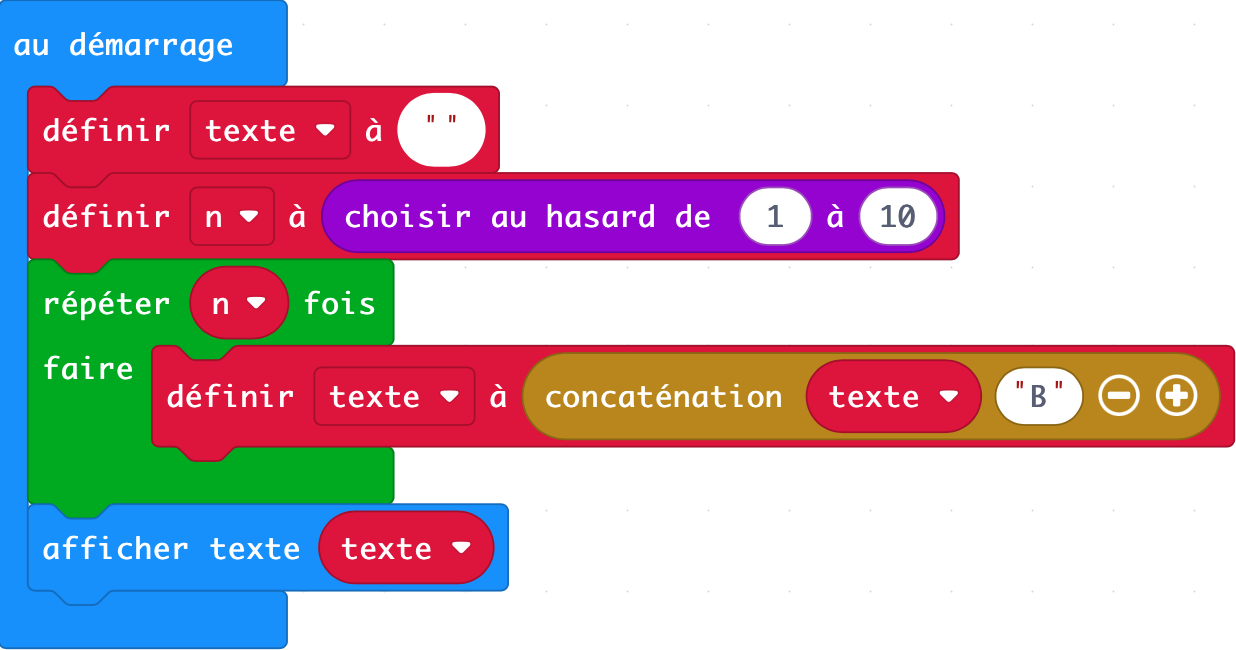
\includegraphics[scale=.5]{ch6_images/var_30}
\end{center}
\end{exercice}


\begin{exercice}
\begin{enumerate}
\item Que fait ce programme si {\it flocon\_x} = 2?
\item Que fait ce programme si {\it flocon\_x} = 4?
\end{enumerate}
\begin{center}
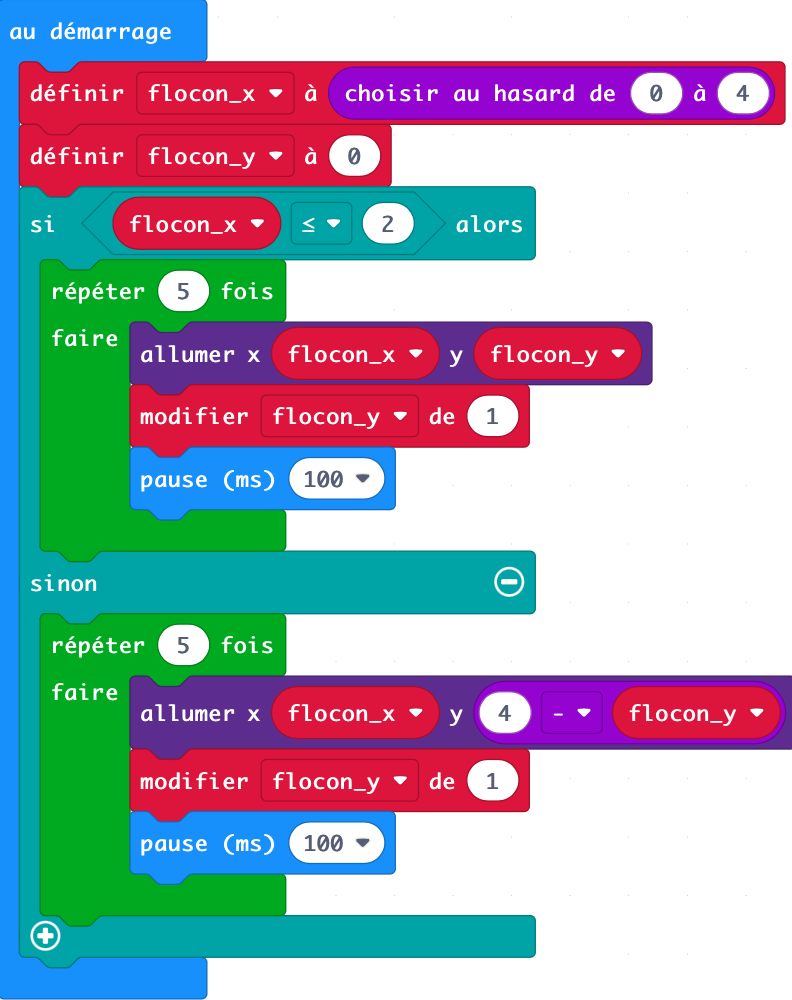
\includegraphics[scale=.5]{ch6_images/var_31}
\end{center}
\end{exercice}

\begin{exercice}
Que fait le programme suivant quand on l'exécute?
\vskip.5cm
\begin{lstlisting}
i = 3
for k in range (7) :
    print(i)
\end{lstlisting}
\vskip.5cm
\end{exercice}

\begin{exercice}
Que fait le programme suivant quand on l'exécute?
\vskip.5cm
\begin{lstlisting}
i = 3
for k in range (7) :
    i = 2 * i
print(i)
\end{lstlisting}
\vskip.5cm
\end{exercice}

\begin{exercice}
Que fait le programme suivant quand on l'exécute?
\vskip.5cm
\begin{lstlisting}
i = 5
n = 10
for k in range (n) :
    print(i)
    i = i + 1
\end{lstlisting}
\vskip.5cm
\end{exercice}

\subsection{La boucle {\it tant que} (while)}

{\it répéter} est une structure de répétition qui ne nous permet pas de faire "efficacement" toutes les répétitions, ou boucles, que nous rencontrons en programmation. Pour palier à cette difficulté, deux autres structures se rencontrent souvent: la boucle {\it tant que } (while) et la boucle {\it pour} (for). Nous allons voir dans ce chapitre la première.

Le format de la boucle {\it tant que} se présente sous la forme:

\ 

\hskip+5cm {\it tant que} {\bf condition est vraie}

\hskip+6cm faire une certaine séquence d'instructions



\vskip+.5cm

La {\bf condition} consiste souvent à vérifier qu'une variable ne dépasse pas une certaine valeur. Il faudra alors {\bf incrémenter} cette variable avant chaque répétition de la boucle. Lorsque cette valeur est dépassée, on sort de la boucle. 

\subsubsection{{\it repeat} et {\it while}}

Il est souvent assez facile de passer d'une boucle {\it tant que} à une boucle {\it répéter}. Par exemple,
les deux programmes suivants, utilisant les structures de répétition {\it répéter} et {\it tant que} sont équivalents:

\begin{multicols}{2}
\begin{center}
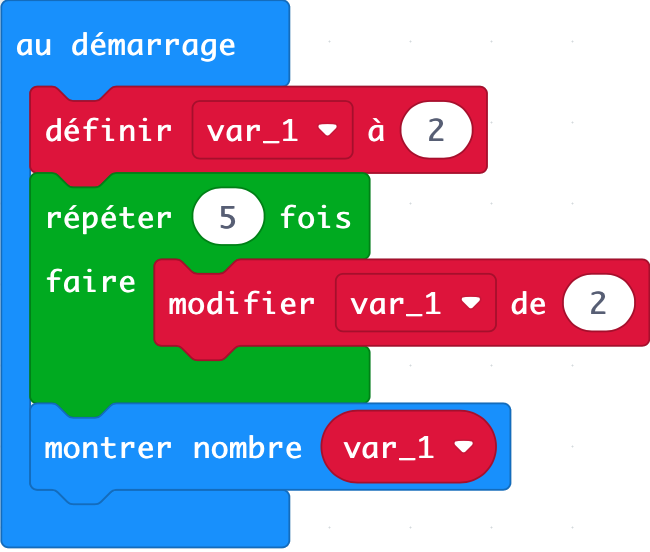
\includegraphics[scale=.5]{ch6_images/var_32}
\end{center}

\begin{center}
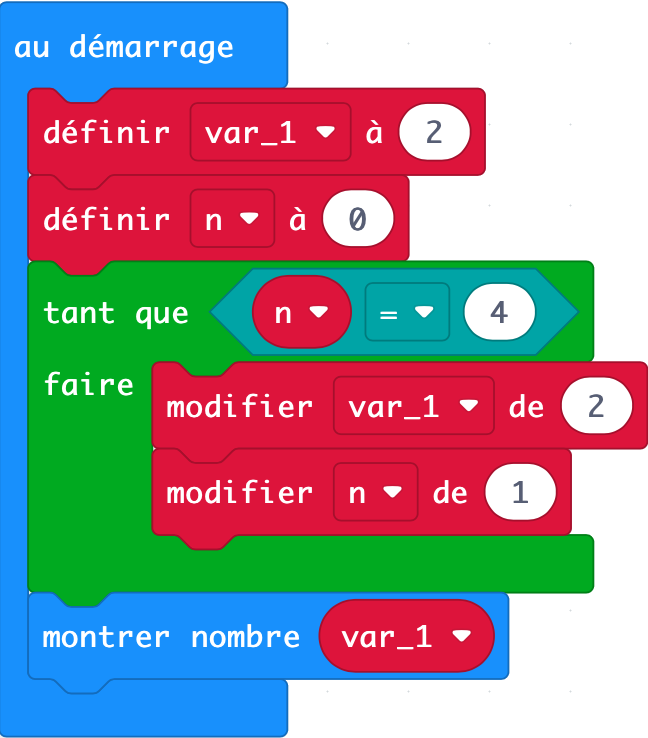
\includegraphics[scale=.5]{ch6_images/var_33}
\end{center}
\end{multicols}


\subsubsection{En Python}

Pour montrer comment on utilise la boucle {\it while} en Python, on va partir d'une situation concrète: Alice gagne 1200.- par mois. Et son salaire monte de 130.- par mois. Bob gagne lui 2900.- par mois, et son salaire augment de 70.- par mois. Combien de mois faudra-t-il pour qu'Alice gagne plus que Bob?

Il existe bien sur des techniques mathématiques pour résoudre ce problème mais nous pouvons aussi représenter la situation par un programme. Nous aurons une variable pour chacun des salaires d'Alice et Bob, et une variable qui compte le nombre de mois, et qui vaudra au début 0. On va répéter nos calculs mensuels tant que le salaire d'Alice est plus petit que le salaire de Bob. Et chaque fois, on va calculer les nouveaux salaires d'Alice et de Bob et ajouter un mois en plus. Ce qui donne:


\vskip.5cm
\begin{lstlisting}
salaire_alice = 1200
salaire_bob = 2900
nombre_de_mois = 0
while salaire_alice <= salaire_bob:
    salaire_alice = salaire_alice + 130
    salaire_bob = salaire_bob + 70
    nombre_de_mois = nombre_de_mois + 1
print(nombre_de_mois)
\end{lstlisting}
\vskip.5cm

Il faudra faire attention lorsqu'on écrit une boucle {\it while} à ne pas avoir une condition qui demeure toujours vrai, sinon le programme ne s'arrêter jamais.

\subsubsection{Exercices}

\begin{exercice}
Que fait le programme suivant?
\begin{center}
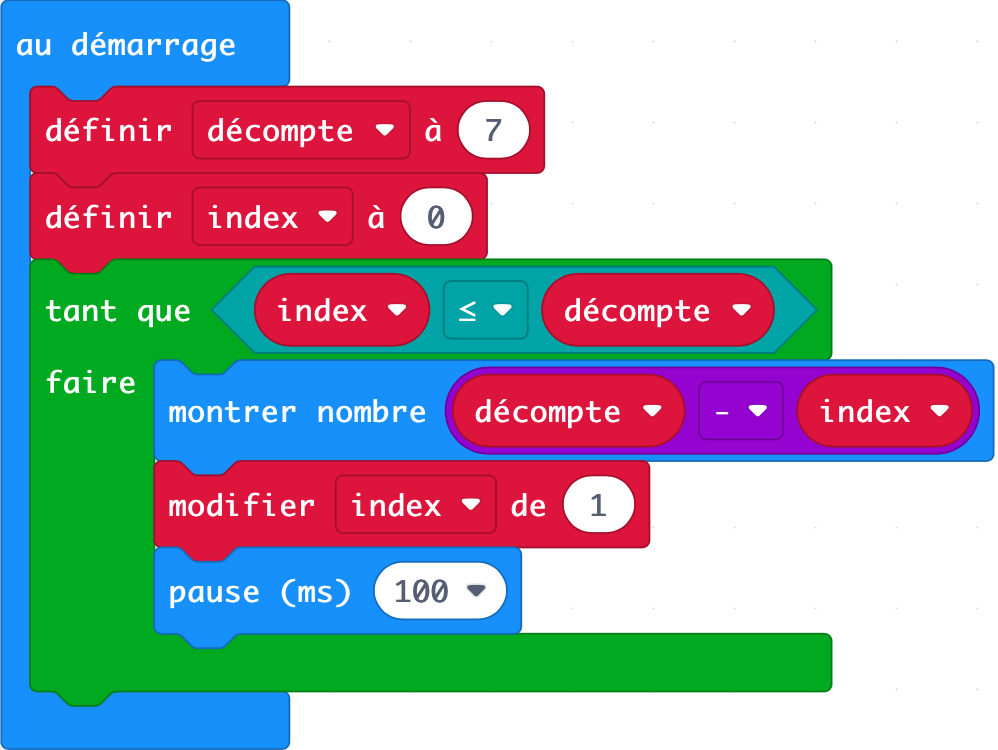
\includegraphics[scale=.4]{ch6_images/var_34}
\end{center}
\end{exercice}

\begin{exercice}
Que fait le programme suivant?
\begin{center}
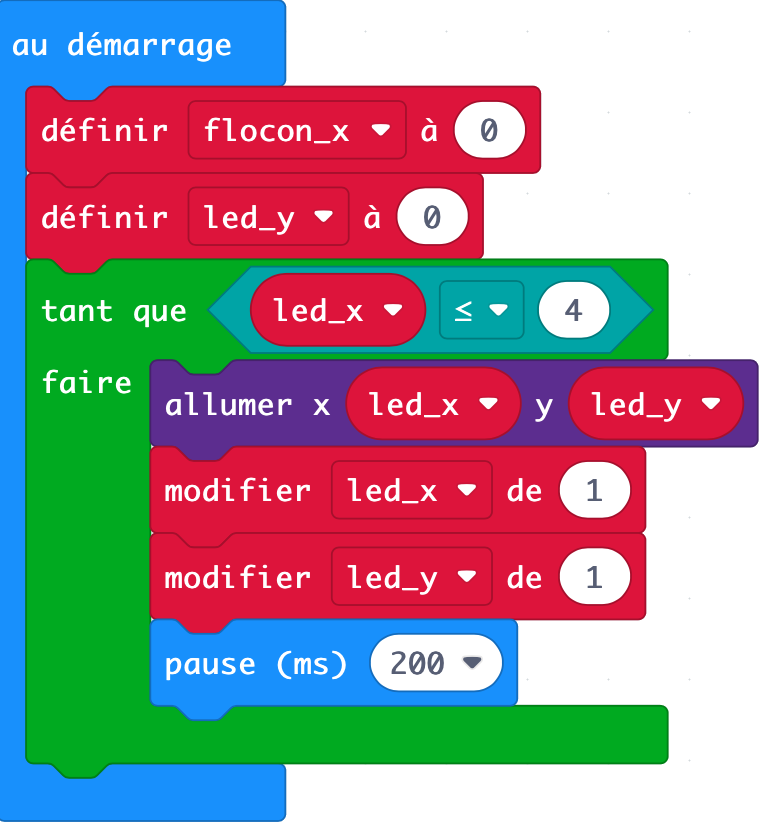
\includegraphics[scale=.4]{ch6_images/var_35}
\end{center}
\end{exercice}

\begin{exercice}
Que fait le programme suivant?
\begin{center}
\includegraphics[scale=.4]{ch6_images/var_36}
\end{center}
\end{exercice}





\begin{exercice}
Que fait le programme suivant quand on l'exécute?
\vskip.5cm
\begin{lstlisting}
n = 2
compteur = 0
limite = 100
while n < limite :
    n = 2 * n
    compteur = compteur + 1
print(compteur)
\end{lstlisting}
\vskip.5cm
\end{exercice}



\begin{exercice}
\vskip.5cm
\begin{lstlisting}
abo_a = 50
abo_b = 0
nombre_seances = 0
while abo_b < abo_a :
    abo_a = abo_a + 9
    abo_b = abo_b + 15
    nombre_seances = nombre_seances + 1
print(nombre_seances)
\end{lstlisting}
\vskip.5cm
\end{exercice}


\begin{exercice}
\vskip.5cm
\begin{lstlisting}
x = 0
n = 10
compteur = 0
while x < n :
    z = 0
    while z < x :
        compteur = compteur + 1
        z = z + 1
    x = x + 1
print(compteur)
\end{lstlisting}
\vskip.5cm
\end{exercice}

\end{document}

